\chapter{Region Based CNN (R-CNN)}

R-CNN (Region based CNN) are used for object detection. Another network also used for objection detection is YOLO (You only look once)

\section{R-CNN (do not use this method, deprecated)}

\begin{figure}[h]
  \centering
  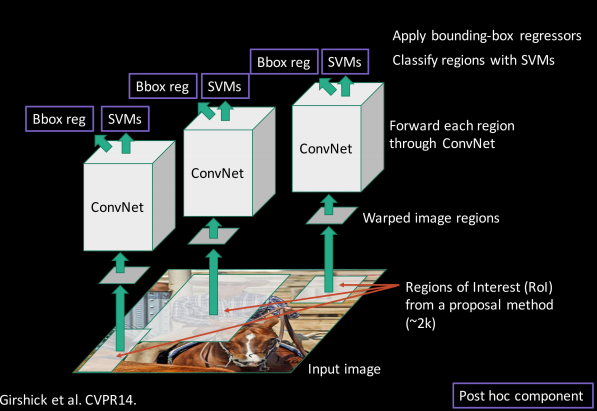
\includegraphics[width=0.6\textwidth]{Images/region_based_cnn/1.png}
  \caption{R-CNN}
\end{figure}
So the idea for object detection is to use R-CNN. First run a region proposal algorithm to obten regions of interets. Then, warp this regions into a fixed size and run the ConvNet with regression head and classification head. The regression head objective is to output an offset to correct "slightly wrong" region proposals.

R-CNN probelms:
\begin{itemize}
\item Slow at test-time: need to run full forward pass of CNN for each region proposal
\item SVMs and regressors are post-hoc: CNN features not updated in response to SVMs and regressors
\item Complex multistage training pipeline
\end{itemize}


Train a R-CNN

1.- \textbf{Train} (or download) a classification model (e.g. AlexNet).
\begin{figure}[h]
  \centering
  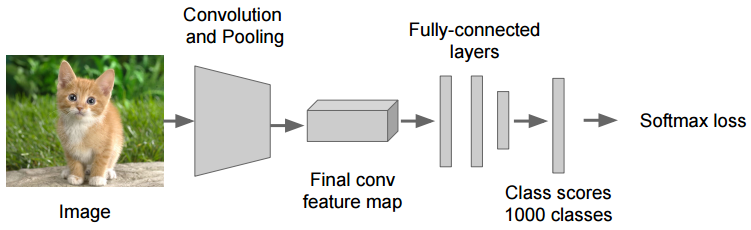
\includegraphics[width=0.6\textwidth]{Images/region_based_cnn/2.png}
  \caption{Train}
\end{figure}
2.- \textbf{Fine-tune model for detection}. Instead of X classes you want Y classes + background. To do so, throw away the final fully-connected layer, add the new one and retrain using positive/negative regions from detection images.
\begin{figure}[h]
  \centering
  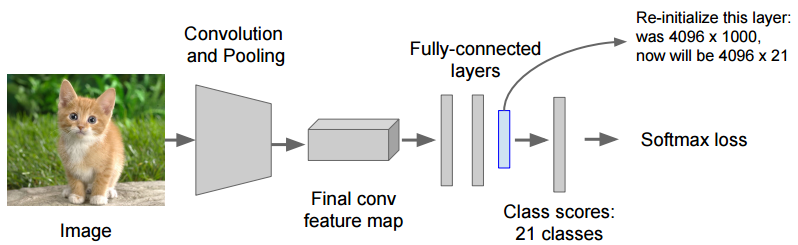
\includegraphics[width=0.6\textwidth]{Images/region_based_cnn/3.png}
  \caption{Fine-tune}
\end{figure}
3.- \textbf{Extract features}. Extract region proposals for all images. For each region: warp to CNN input size, run forward through CNN, save last pool features to disk.
\begin{figure}[h]
  \centering
  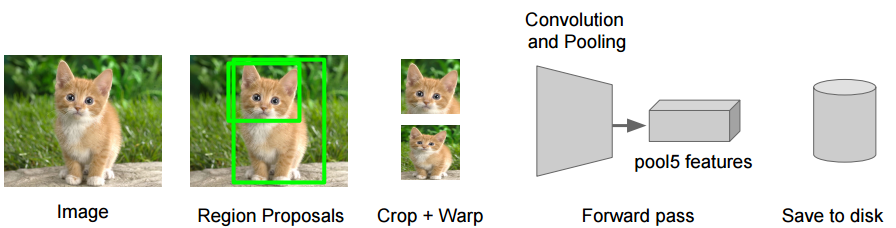
\includegraphics[width=0.6\textwidth]{Images/region_based_cnn/4.png}
  \caption{Extract features}
\end{figure}
4.- \textbf{Train classification head}. Train one binary SVM per class using as input the saved features from last step.

5- \textbf{Train regression head}. For each class, train a linear regression model to map from cached features to offset to GT boxes to make up for "slightly wrong" proposals of the region proposals.
\begin{figure}[h]
  \centering
  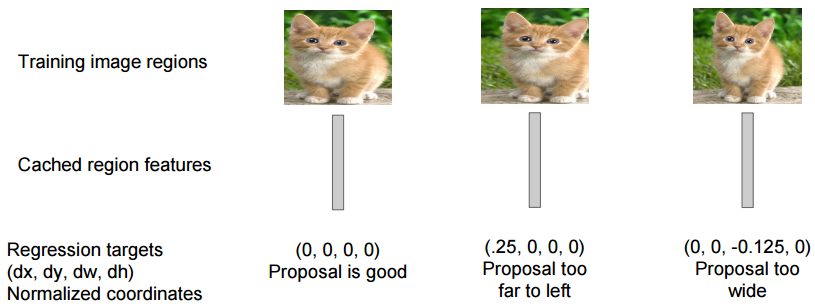
\includegraphics[width=0.6\textwidth]{Images/region_based_cnn/5.png}
  \caption{Train regression head}
\end{figure}
\begin{figure}[h]
  \centering
  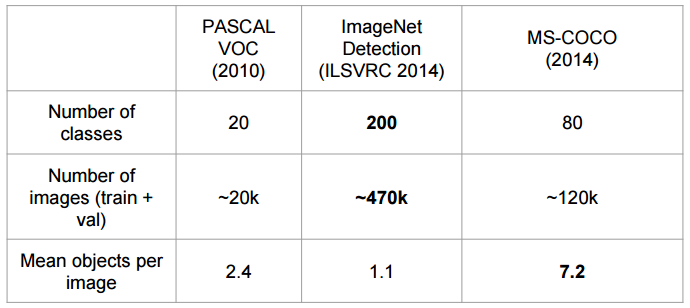
\includegraphics[width=0.6\textwidth]{Images/region_based_cnn/6.png}
  \caption{Usual datasets for training}
\end{figure}



\section{Fast R-CNN (do not use this method, deprecated)}
A new proposal called Fast R-CNN appeared trying to solve R-CNN problems. The idea is just to swap the order of extracting regions of interest and features. Still, no sliding windows.

\begin{figure}[h]
  \centering
  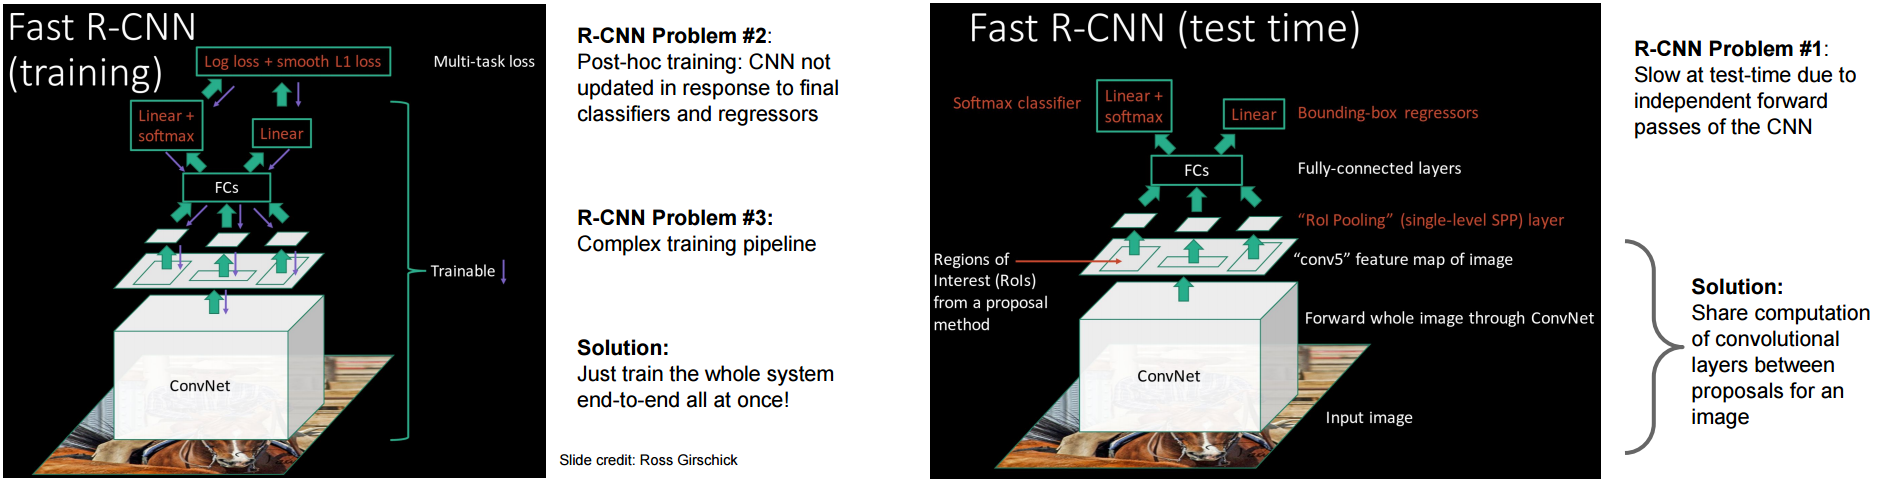
\includegraphics[width=\textwidth]{Images/region_based_cnn/10.png}
  \caption{Fast R-CNN training/testing time}
\end{figure}

\subsection*{The only mystery here are region of interest pooling.}

The HxW image is processed by the convolution and pooling part and regions of interest are proposed (with an external algorithm). The problem now is that the FC layer is expecting a fixed size input. To solve this, given the region proposal, we project it onto the conv feature map, divide it into hxw grid and do max-pool within each grid cell.

\begin{figure}[h]
  \centering
  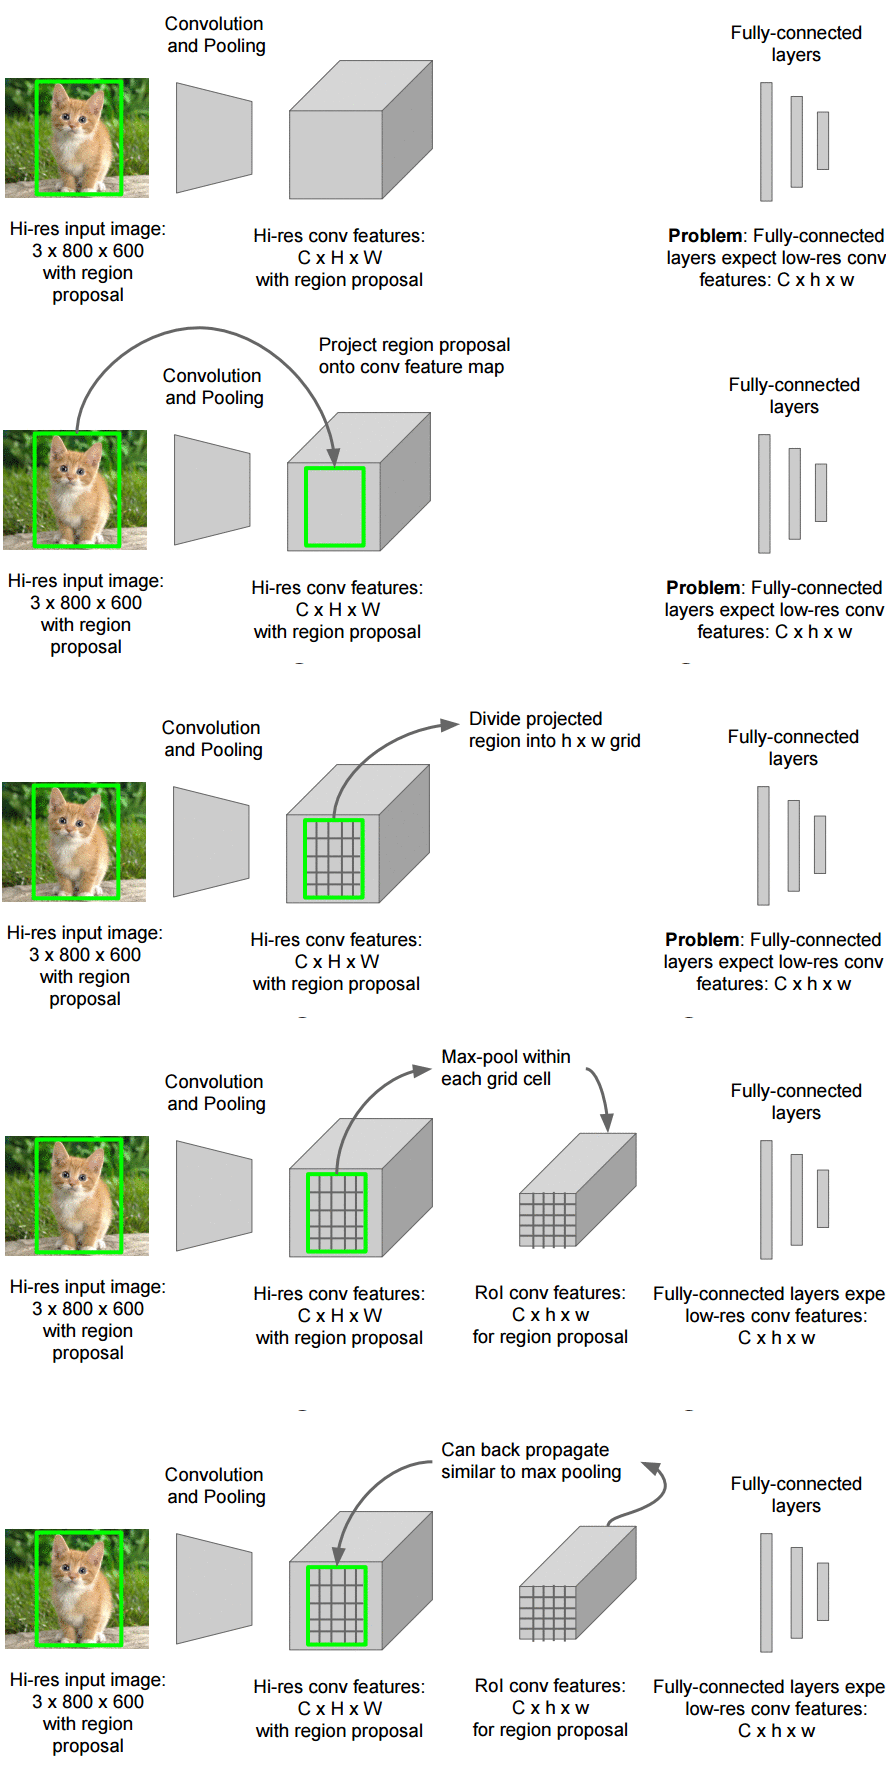
\includegraphics[width=0.6\textwidth]{Images/region_based_cnn/9.png}
  \caption{process}
\end{figure}

With this simple straggly the FC layer will always receive the same input size.  Moreover, we can backprop through this strategy with no problem because it only uses max-pool.

In terms of mAP (accuracy) is more or less the same
The computational time improvement of Fast R-CNN w.r.t. R-CNN is impressive:
\begin{itemize}
\item x8.8 training time speed up
\item x25 testing time speed up (50s to 2s)
\end{itemize}

However, the bottleneck is extracting the regions with a region proposals algorithm. Without it, the speed would be:
\begin{itemize}
\item x146 testing time speed up (47s to 0.32s)
\end{itemize}

so why not extracting the ROIs with the CNN? this is what Faster R-CNN proposes

\section{Faster R-CNN}

To solve the problem of region proposals algorithm botleneck in Fast R-CNN, Faster R-CNN proposes to extract the regions of interest with another network using the information of the last layer of the CNN net.

Insert a Region Proposal Network (RPN) after the last convolutional layer.

RPN trained to produce region proposals directly; no need for
external region proposals!

After RPN, use RoI Pooling and an upstream classifier and bbox regressor just like Fast R-CNN

Still, the Rol pooling does not allow to introduce rotations into your regions of interests. To introduce rotations, a DeepMind paper proposes to do bilinear interpolation similar computer graphics.

\begin{figure}[h]
  \centering
  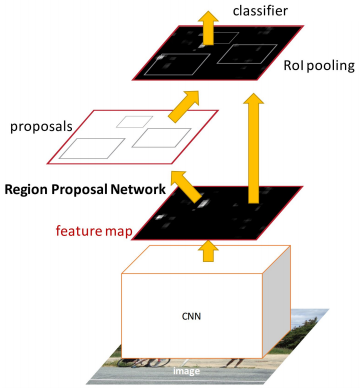
\includegraphics[width=0.4\textwidth]{Images/region_based_cnn/14.png}
  \caption{Faster R-CNN}
\end{figure}

\subsection*{The cool thing here is the region proposal network, how does it work?}

Build a small network for:

\begin{itemize}
\item Classifying object or no-object, and
\item Regressing bbox locations
\end{itemize}

Use N anchor boxes at each location. Anchors are translation invariant: use the same ones at every location. For all the feature map points, at the original input image apply all anchors to the point corresponding to the current feature map point. So we take as features the convolutional feature map region corresponding to the anchor region in the original image.

For each of this anchor boxes it produces a score weather there is an object or not; and a finer localization with reference to the anchor (they are an offset to the anchor boxes)

So you are learning different weights for each anchor.

\begin{figure}[h]
  \centering
  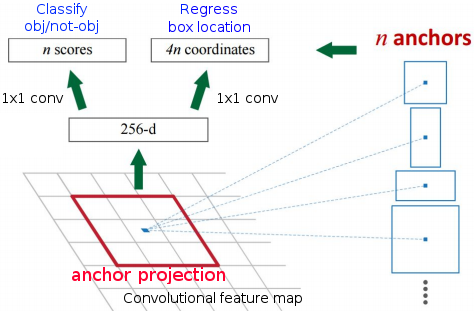
\includegraphics[width=0.6\textwidth]{Images/region_based_cnn/11.png}
  \caption{The cool thing here is the region proposal network, how does it work?}
\end{figure}

\subsection*{How to train it?}

To train it, in some unpublished work, it trains the net as a net with 4 losses

One network, four losses
\begin{itemize}
\item RPN classification (anchor good / bad)
\item RPN regression (anchor to proposal)
\item Fast R-CNN classification (over classes)
\item Fast R-CNN regression (proposal to box)
\end{itemize}

\begin{figure}[h]
  \centering
  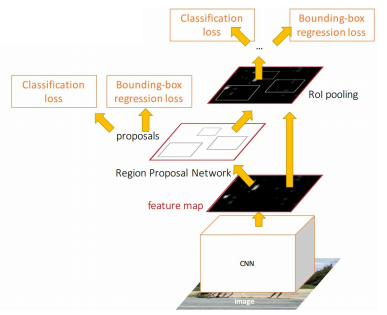
\includegraphics[width=0.6\textwidth]{Images/region_based_cnn/15.png}
  \caption{How to train it?}
\end{figure}

In terms of mAP (accuracy) is more or less the same than with Fast R-CNN
The computational time improvement of Faster R-CNN w.r.t. R-CNN is impressive: x250 testing time speed up (50s to 0.2s)

